\underbar{\textbf{\large Ejercicio 1:}} Se dispone de una clase base Persona y dos clases especializadas Alumno y Profesor. Se quiere saber qué alumnos están matriculados en qué asignaturas y qué profesores imparten qué asignaturas, y viceversa. 

Para ello hay dos opciones:
\begin{itemize}
  \item Dos asociaciones bidireccionales varios a varios, una entre Alumno y Asignatura, y otra entre Profesor y Asignatura.
  \item Una única asociación bidireccional varios a varios entre las clases Persona y Asignatura.
\end{itemize}
Como queremos que solamente accedan a las asignaturas ya sean Alumnos o Profesores si lo implementamos mediante la segunda manera cualquier Persona que no sea ni Alumno ni Profesor podrá acceder a las asignatura, como eso es algo que no queremos lo implementaremos mediante la primera manera.

\begin{figure}[h]
  \begin{center}
    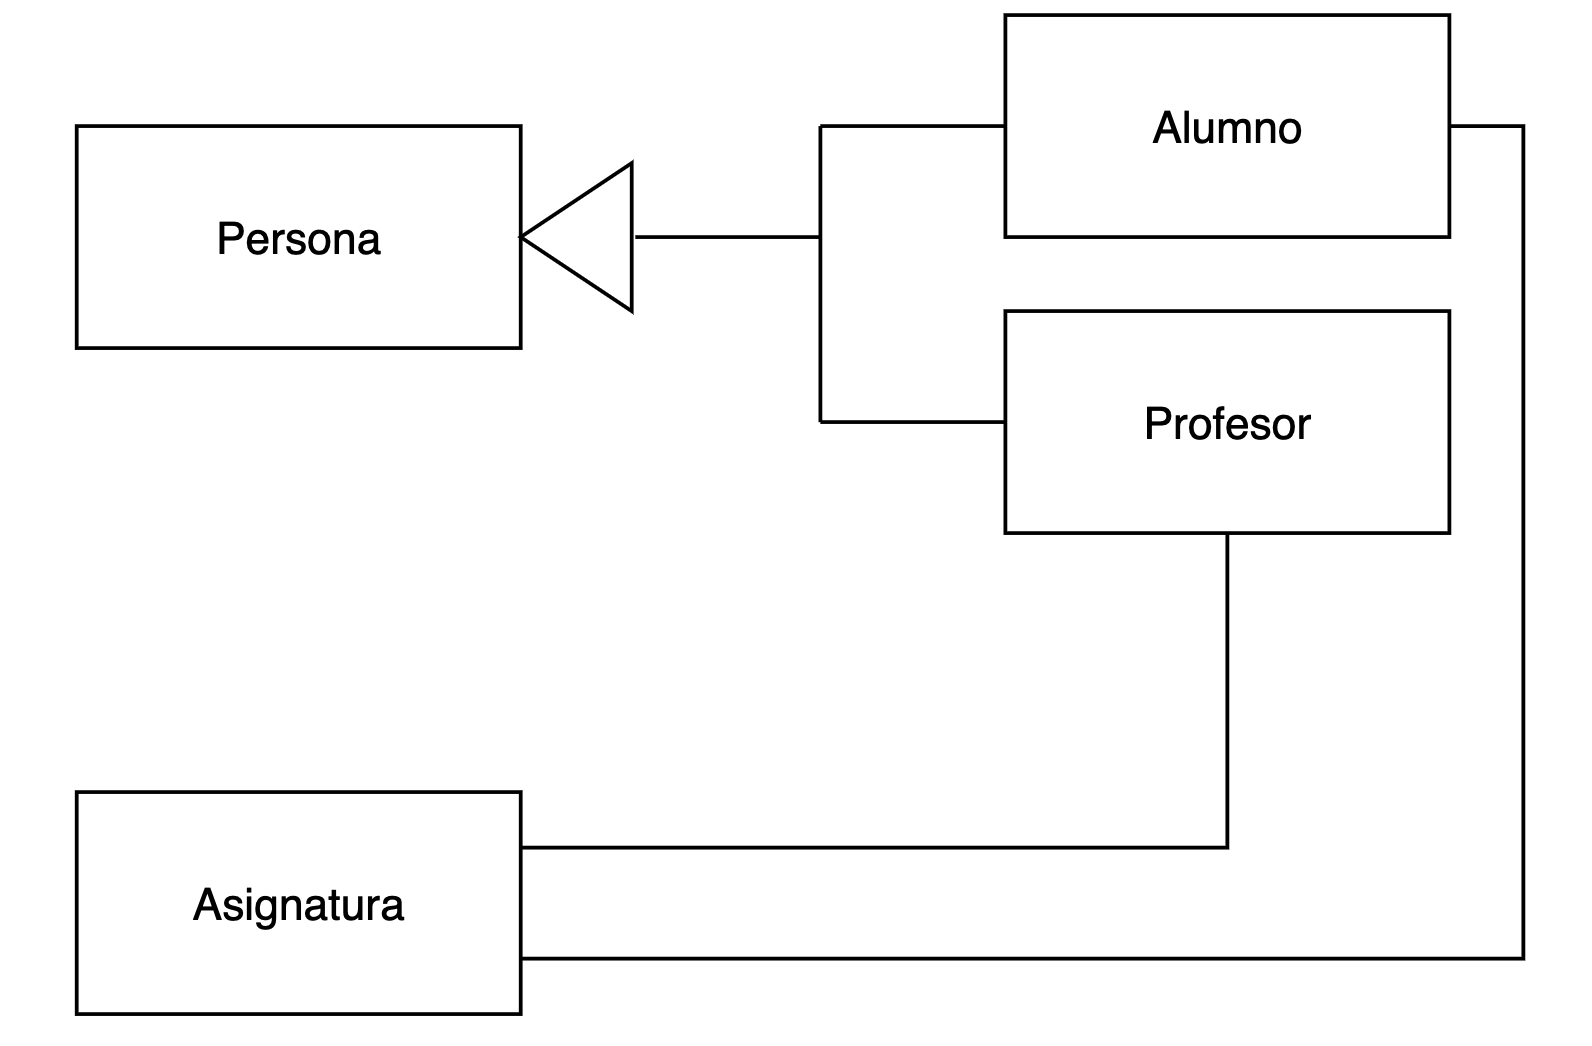
\includegraphics[width=\textwidth]{assets/Seminario3_2_1.png}
  \end{center}
  \caption{Resultado de la implementación del ejercicio}
\end{figure}
\newpage
\underbar{\textbf{\large Ejercicio 2:}} Supóngase que existen ya definidas dos clases Ventana (ventana gráfica), y Barra (barra de desplazamiento) y se quiere definir una nueva clase VentanaBarra (ventana con barra de desplazamiento). Indique si definiría la nueva clase utilizando alguna de las anteriores o como una nueva clase independiente. En caso de utilizar alguna de las ya definidas explique qué relaciones son las que se establecen entre ellas y cómo las codificaría. Razone la respuesta.

Una VentanaBarra estará compuesta por una Ventana y una Barra, por tanto, podriamos implementarla como dos composiciones 1-1:
\begin{minted}[breaklines]{C++}
class Ventana{};
class Barra{};
class VentanaBarra : public Ventana, private Barra{
  public:
    VentanaBarra(Ventana& v, Barra& b):Ventana(v),Barra(b){}
};
\end{minted}

\underbar{\textbf{\large Ejercicio 3:}} Dadas las clases A y B, indicar qué asignaciones son correctas:
\begin{figure}[h]
\begin{minipage}{0.35\textwidth}
\begin{lstlisting}[frame = single]
class A{};
class B: public A {};
int main() {
  A objA, *pA;
  B objB, *pB;
  pA = &objA;
  pB = &objB;
  objA = objB;
  objA = (A)objB;
  objB = objA;
  objB = (B)objA;
  pA=pB;
  pB=pA;
  pB = (B*)pA;
}
\end{lstlisting}
\end{minipage}
\hfill
\begin{minipage}{0.6\textwidth}
\underbar{Asignaciones:}\\
\textbf{\texttt{pA = \&objA;}}→ Correcta, puntero pa de tipo A apunta a un objeto de A.\\
\textbf{\texttt{pB = \&objB;}}→ Correcta, puntero pb de tipo b apunta a un objeto de B. \\
\textbf{\texttt{objA = objB;}}→ Correcta, conversión de un objeto B a uno A (conversión implícita hacia arriba.)\\
\textbf{\texttt{objA = (A)objB;}}→ Correcta, conversión de un objeto B a uno A (conversión explícita).\\
\textbf{\texttt{objB = objA;}}→ Error, no se pueden convertir objeto de A a B de forma implícita.\\
\textbf{\texttt{objB = (B)objA;}}→Error, no se pueden convertir objetos de A a B de forma explícita. \\
\textbf{\texttt{pA=pB;}}→Correcto, conversión de puntero de B a A implícitamente.\\
\textbf{\texttt{pB=pA;}}→ Error, no se puede convertir un puntero de A a B implicitamente. \\
\textbf{\texttt{pB = (B*)pA;}}→ Correcta, conversión explicita de puntero de A a uno de B (asignación de punteros del mismo tipo).\\

\end{minipage}
\end{figure}
\newpage
\underbar{\textbf{\large Ejercicio 4:}} Sea cierta clase base B y una derivada D. Ambas tienen definido un cierto método f(). Diga si el siguiente código es correcto y a qué método f() se llamaría.
\begin{figure}[h]
  \begin{minipage}{0.2\textwidth}
    \begin{lstlisting}[frame = single]
  B b, *bp;
  D d, *dp;

  b.f();

  bp=&d;
  bp->f();

  dp=&d;
  dp->f();  
    \end{lstlisting}
  \end{minipage}
\hfill
\begin{minipage}{0.75\textwidth}
 \underbar{Método f() que se llamaría:}\\
  \textbf{\texttt{b.f();}}→ Vemos que b es un objeto de B (base), se llama a f() de B. \\
  \textbf{\texttt{pb ->f();}}→ Vemos que previamente una referencia de un objeto D (derivada) es apuntada por un puntero B (base), como la clase Base no es polimorfica nos fijamos en el tipo del puntero, por tanto , se llama a f() de B. \\
  \textbf{\texttt{dp -> f();}}→ Vemos que dp es un puntero que apunta a la referencia de un objeto de D, como no cambia de tipo, se llama a f() de D.\\

\end{minipage}
\end{figure}

\underbar{\textbf{\large Ejercicio 5:}} Dadas las siguientes declaraciones:
\begin{lstlisting}[frame = single]
  struct A{int a;};
  struct B:public A{int b;};
  struct C:public A{int c;};
  struct D:public B,public C{int d;} v;
\end{lstlisting}

1. ¿Cuántos miembros tiene el objeto v? ¿Cómo se accede a cada uno de ellos?

El objeto v tiene 5 miembros, y se acceden de la manera: \texttt{d.v}, \texttt{c.v}, \texttt{b.v},\texttt{v.B::a}, \texttt{v.C::a}.

Vemos que tiene dos miembros de la clase A repetidos, esto crea una ambigüedad, por tanto, para solucionar esto hacemos que tanto la clase B como C herenden virtualmente de A, haciendo que tenga solamente 4 miembros. Los dos últimos desaparcen y al miembro de la clase A se accedería de la manera \texttt{v.a}.